%-------------------------------------------------------------------------------
%                            BAB III
%               		METODOLOGI PENELITIAN
%-------------------------------------------------------------------------------
\fancyhf{} 
\fancyfoot[C]{\thepage}
\chapter{METODOLOGI PENELITIAN}

\section{Waktu dan Lokasi Penelitian}
Penelitian ini akan bertempat pada Gedung A Fakultas Matematika dan Ilmu Pengetahuan Alam. Waktu yang dibutuhkan agar penelitian ini dapat diimplementasikan adalah 4 bulan terhitung dari Juni 2022 hingga September 2022.

\section{Alat dan Bahan}
Alat dan Bahan yang akan digunakan pada penelitian ini terdiri dari beberapa perangkat keras (\textit{Hardware}) dan perangkat lunak (\textit{Software}) yang dijabarkan sebagai berikut:

\begin{enumerate}
\item Perangkat Keras
	\begin{itemize}
	\item Laptop Acer Aspire E5-475g dengan RAM 16GB, Intel Core i5-7200U 2.5GHz, Nvidia GeForce 940MX 2GB, \textit{Harddisk} (HDD) 1500Gb, \textit{Solid State Drive} (SSD) 250GB.
	\item \textit{Smartphone} Xiaomi Poco F3 dengan RAM 6GB, \textit{Internal Storage} 128GB.
	\item \textit{Personal Computer} dengan AMD Ryzen 7 2700x, RAM 16GB, Nvidia GeForce RTX 2080 8GB, \textit{Solid State Drive} (SSD) 500GB.
	\item \textit{Beacon Bluetooth}.
	\end{itemize}

\item Perangkat Lunak
	\begin{itemize}
	\item Windows 11 Pro
	\item Linux Ubuntu 20.04.1 LTS
	\item Android Studio 2021.2.1.15
	\item Visual Studio Code
	\item Figma
	\item Notion
	\item Vosk API
	
	\end{itemize}
\end{enumerate}

\section{\textit{Roadmap} Penelitian}
\textit{Roadmap} penelitian merupakan diagram yang menggambarkan rangkaian beberapa penelitian yang saling berkesinambungan dalam rentang waktu tertentu. \textit{Roadmap} penelitian biasa dibuat untuk memberikan batasan kepada peneliti agar menghindari pengamatan yang tidak perlu dan fokus terhadap bagian penelitiannya saja. Pada penelitian ini dibagi ke dalam 2 fase. Fase pertama pada tahun 2019 memiliki fokus penelitian pada \textit{indoor localization} dengan menggunakan \textit{Bluetooth Low Energy} (BLE) dan menggunakan \textit{Wireless Local Area Network} (WLAN) dapat dilihat gambar \ref{img:fase1}. Pada fase kedua pada tahun 2020 lebih berfokus pada penelitian \textit{Indoor Localization} dengan menggunakan BLE. Penelitian ini terletak pada fase 2 di tahun 2020 dengan topik utama yaitu Aplikasi Navigasi \textit{Indoor} dengan sub topik untuk pengguna Tunanetra. Penelitian ini memiliki batasan berupa pembangunan aplikasi \textit{mobile} untuk \textit{Route Guidance} untuk Tunanetra, seperti yang ditunjukkan pada gambar \ref{img:fase2} dengan kata yang dicetak tebal berwarna merah sebagai berikut.


\begin{figure}[H]
  \begin{adjustbox}{addcode={\begin{minipage}{\width}}{\caption{%
      \textit{Roadmap} Penelitian Fase 1
      }\label{img:fase1}\end{minipage}},rotate=90,center} %label gambar simpen disetelah capt
      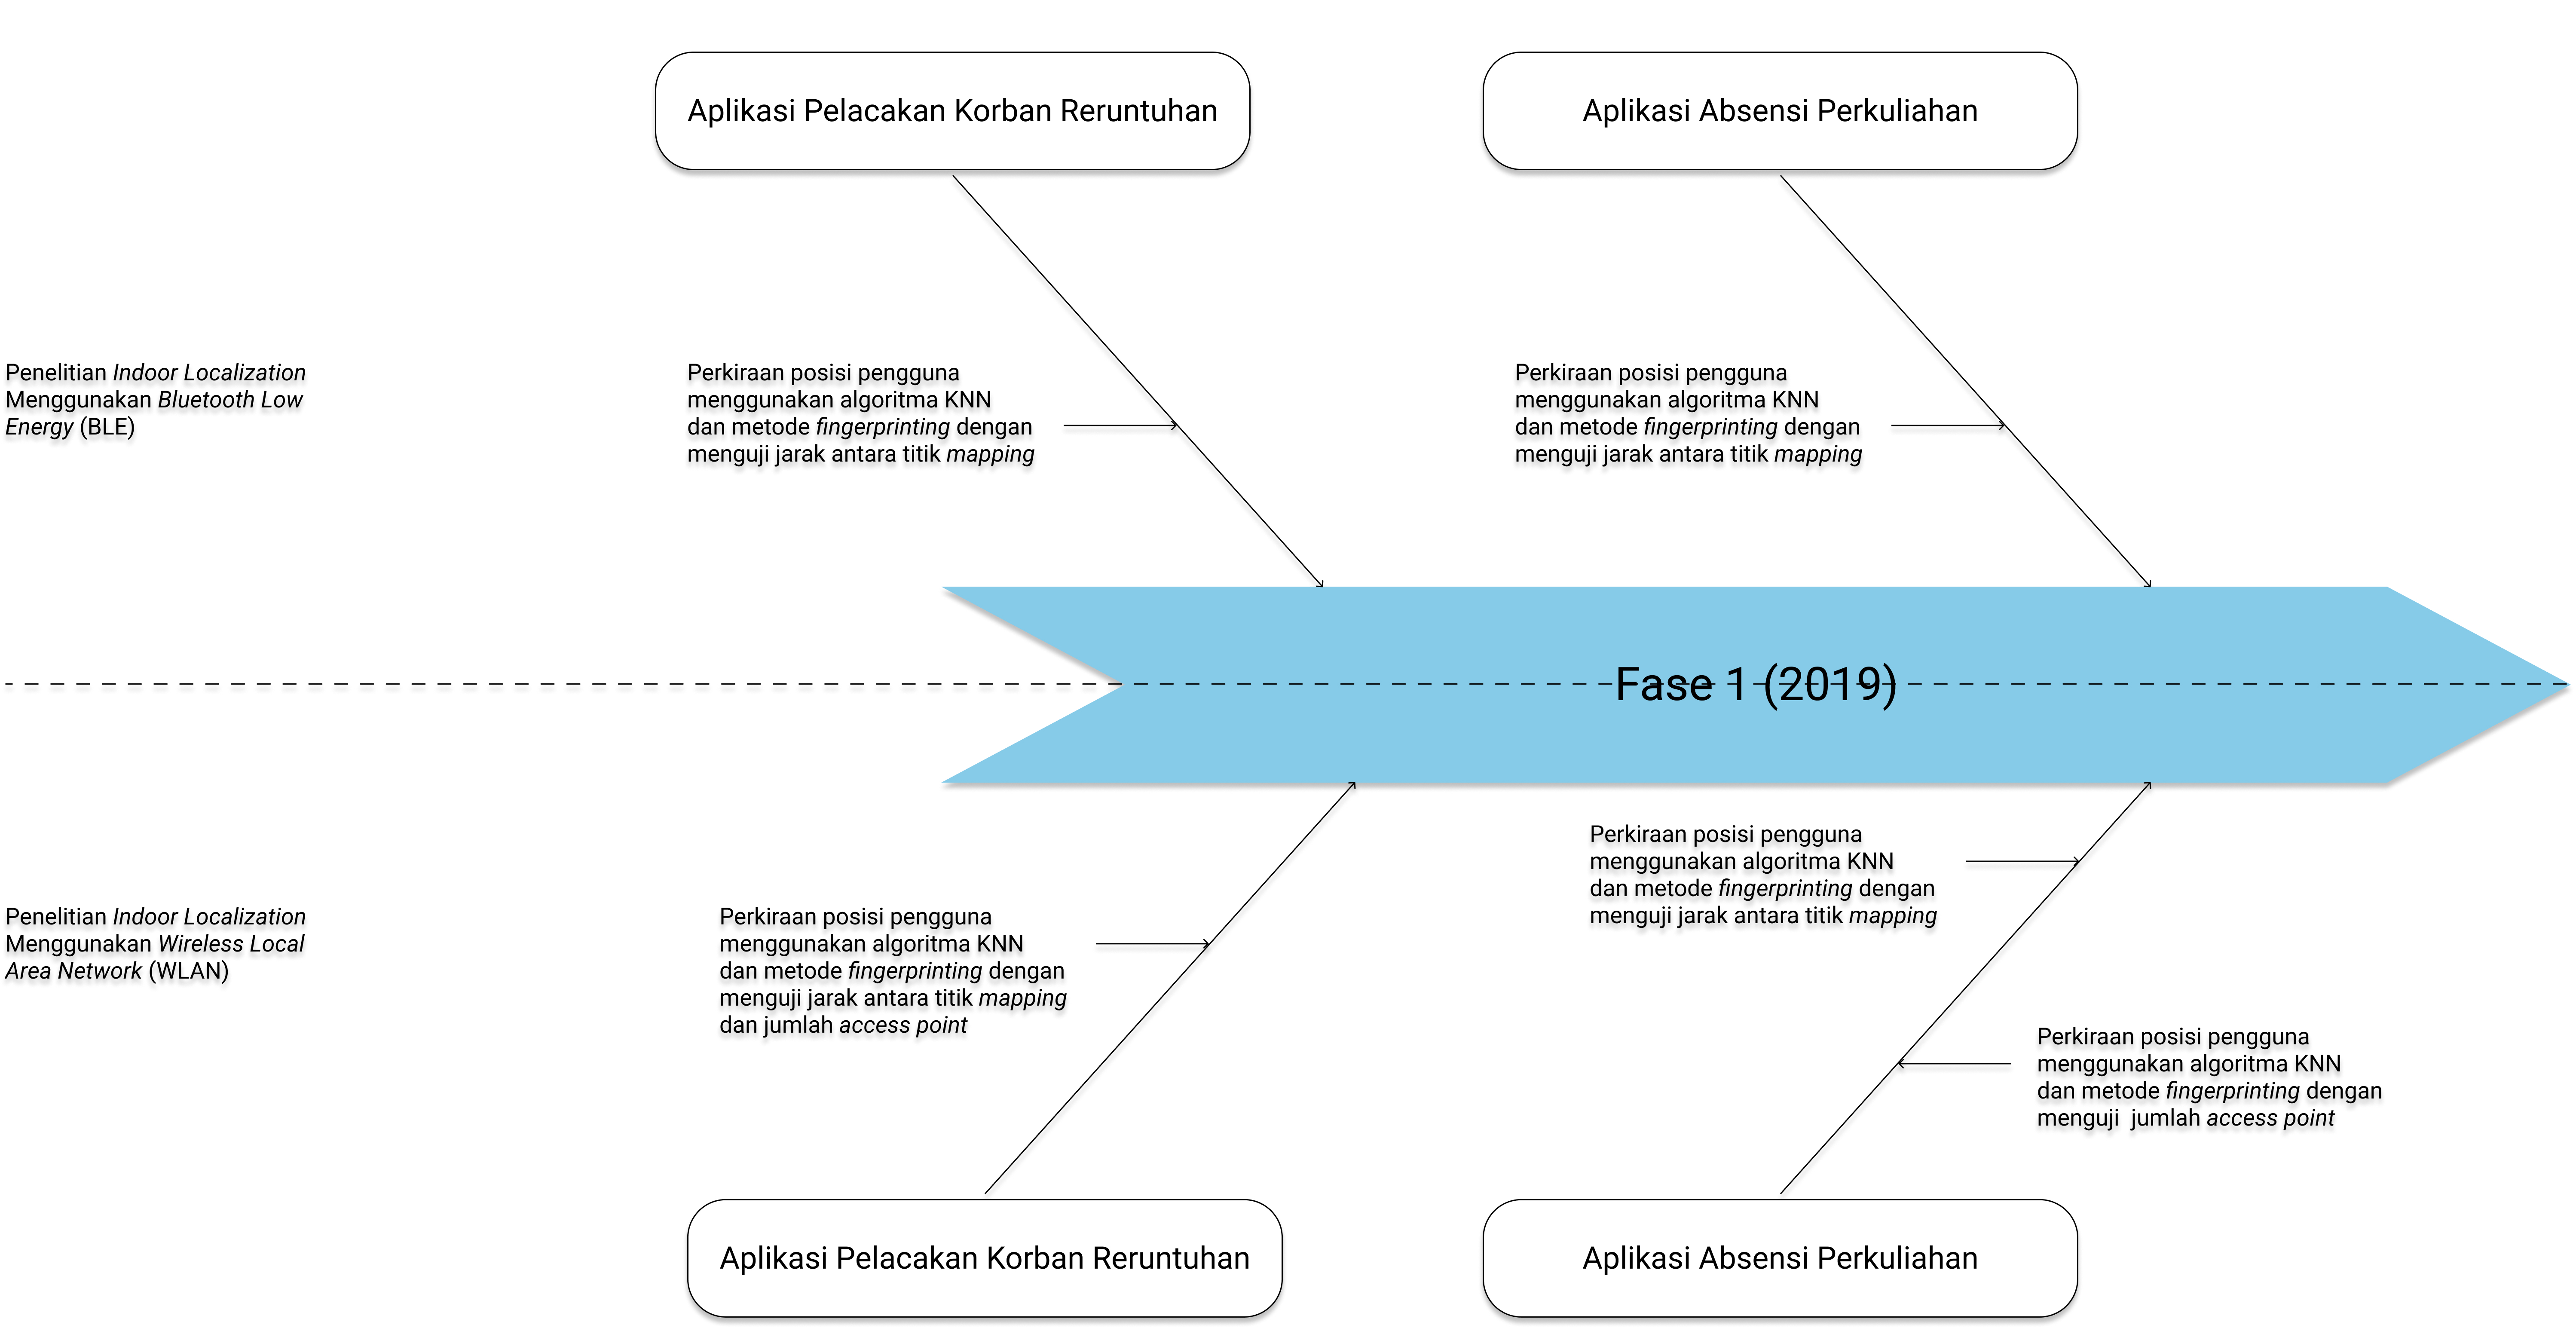
\includegraphics[scale=.3]{gambar/bab3/rp_fase1}%
  \end{adjustbox}
\end{figure}

\fancyhf{} 
\fancyfoot[R]{\thepage}

\begin{figure}[H]
  \begin{adjustbox}{addcode={\begin{minipage}{\width}}{\caption{%
      \textit{Roadmap} Penelitian Fase 2
      }\label{img:fase2}\end{minipage}},rotate=90,center}
      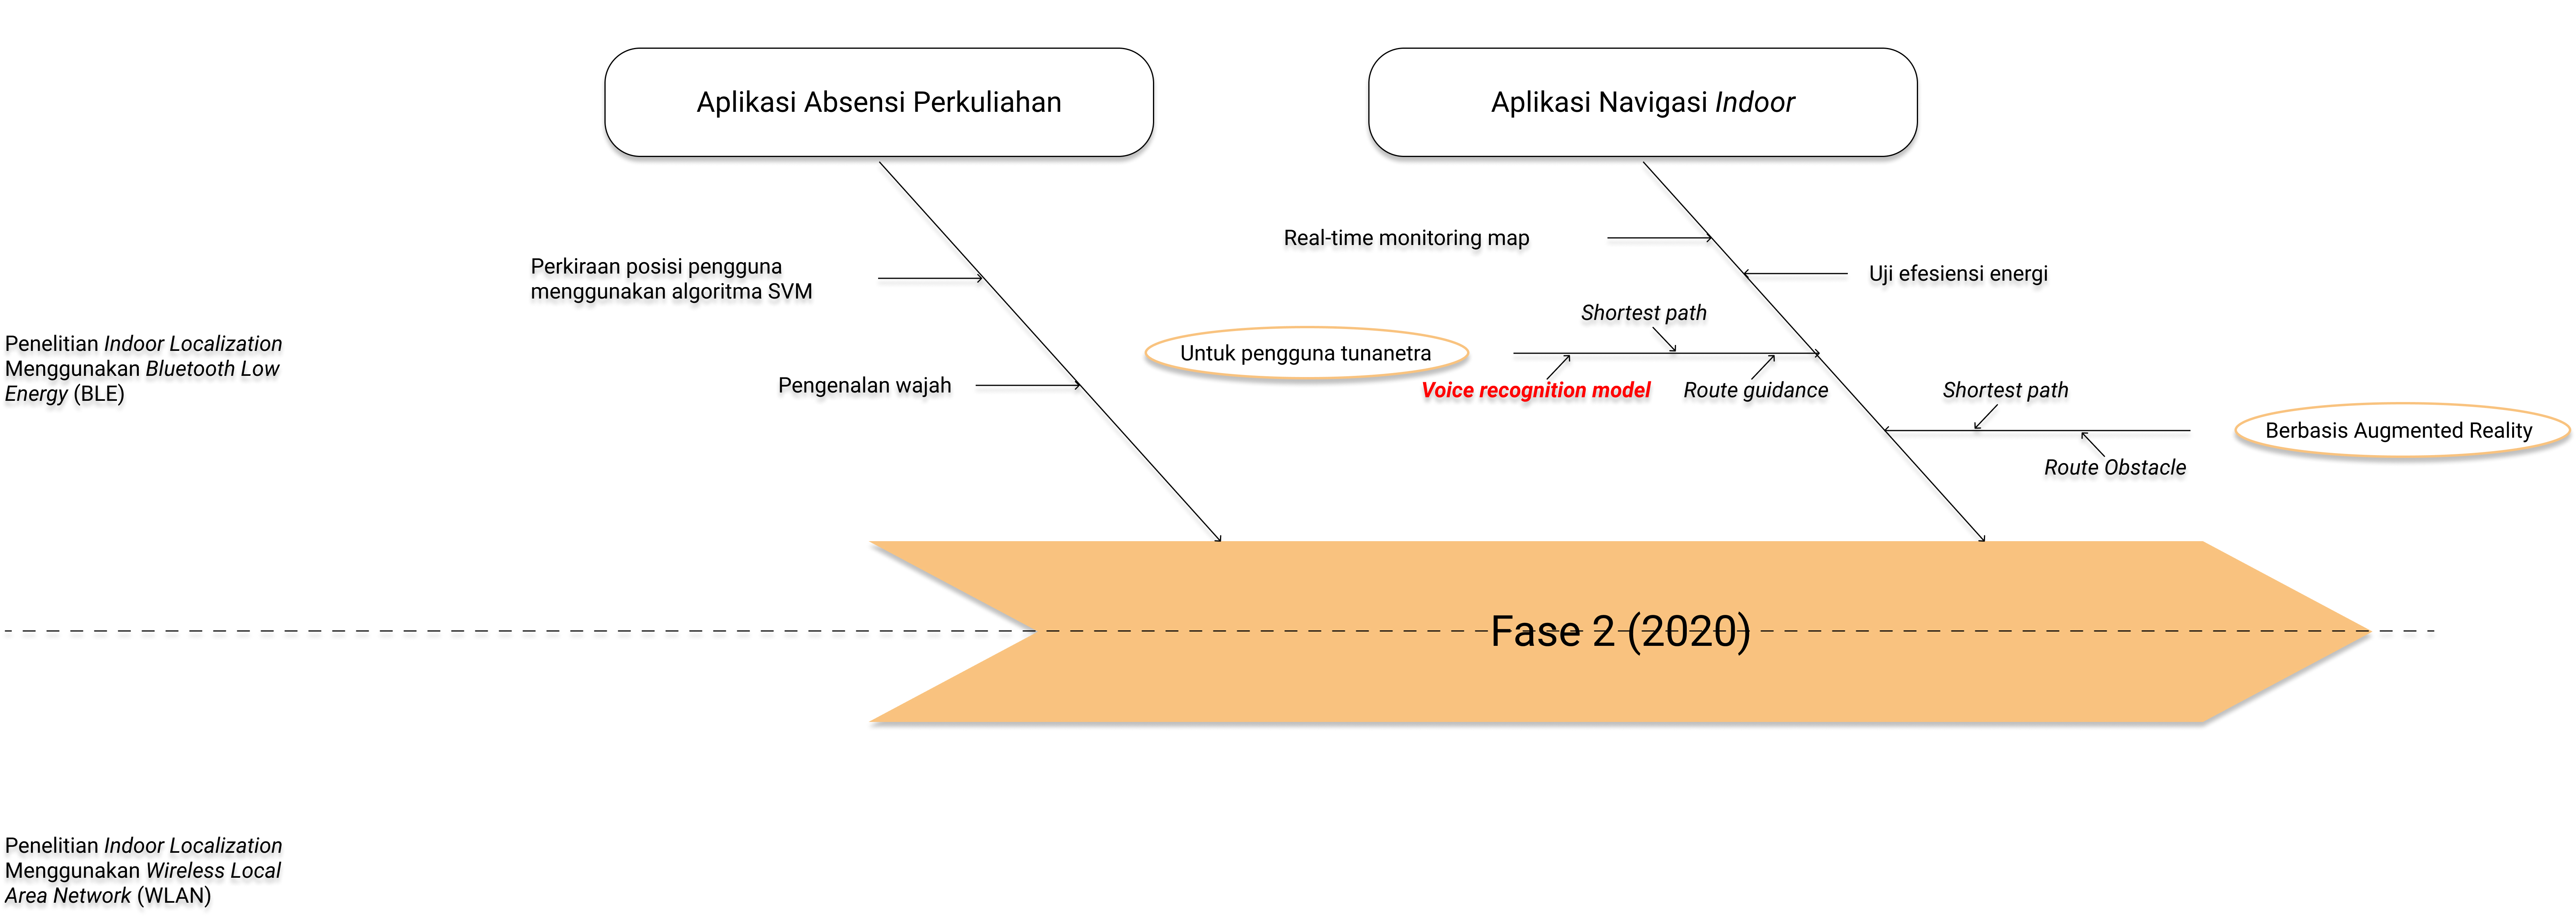
\includegraphics[scale=.3]{gambar/bab3/rp_fase2}%
  \end{adjustbox}
\end{figure}

\fancyhf{} 
\fancyfoot[R]{\thepage}

\section{Metode Penelitian}
Metode penelitian yang dilakukan dalam penelitian ini ditunjukkan pada Gambar \ref{img:diagram_alir_penelitian}.

\begin{figure}[H]
\centering
{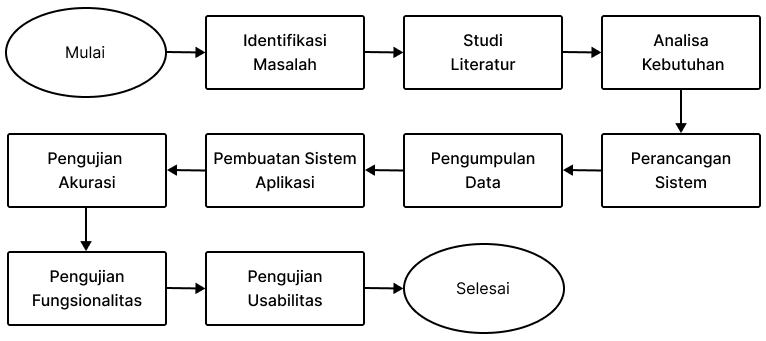
\includegraphics [width = 14cm, height= 8cm]{gambar/bab3/diagram_alir}}
\caption{Diagram Alir Penelitian}
\label{img:diagram_alir_penelitian}
\end{figure}

\fancyhf{} 
\fancyfoot[R]{\thepage}

\subsection{Identifikasi Masalah}
Tahapan ini merupakan tahapan yang dilakukan untuk mengidentifikasi masalah pada lingkungan yang berhubungan dengan aplikasi yang akan dibuat baik secara langsung maupun tidak langsung dan menjadi landasan mengapa aplikasi ini harus dibuat. Masalah-masalah yang berhasil di identifikasi adalah sebagai berikut:

\begin{itemize}
\item Belum ada teknologi Route Guidance System/Wayfinding System berbasis Indoor positioning dengan panduan rute menggunakan Speech Command Recognition di Universitas Syiah Kuala.

\item Membantu Tunanetra menemukan ruangan di Gedung A FMIPA Universitas Syiah Kuala dipandu dengan navigasi suara.

\end{itemize}

%%%%%%%%%%%%%%%%%%%%%%%%%%%%%%%%%%%%%%%%%%%
\subsection{Studi Literatur}
Studi literatur digunakan sebagai bahan referensi selama proses penelitian. Studi literatur dilakukan dengan cara mencari situs website dan jurnal-jurnal terkait tentang penelitian, baik jurnal nasional maupun internasional, buku-buku yang telah diterbitkan, serta situs-situs internet yang berkaitan dengan permasalahan yang dikaji dalam penelitian. Studi literatur dapat dikembangkan untuk menyempurnakan kekurangan dari penelitian sebelumnya.

%%%%%%%%%%%%%%%%%%%%%%%%%%%%%%%%%%%%%%%%%
\subsection{Persiapan Data untuk Kaldi}
Pada tahapan ini ada beberapa file yang harus disiapkan untuk membuat model \textit{speech recognition}, yaitu ada persiapan data akustik untuk membuat \textit{acoustic model} dan \textit{language data} untuk membuat \textit{language model}. Sebelum mempersiapkan beberapa \textit{file} yang dibutuhkan, data suara yang telah dikumpulkan di bagi menjadi 2 bagian, di mana 80\% \textit{speaker} untuk \textit{data training} dan 20\% speaker untuk \textit{data testing}. Berikut adalah penjelasan dari persiapan data akustik dan \textit{language data}:

\begin{enumerate}
\item Persiapan data akustik
\par Pada tahapan ini, ada 5 file yang harus dibuat agar Kaldi dapat memahami data audio yang akan diproses. Berikut adalah penjelasan file yang harus dibuat:
	\begin{itemize}
	\item Spk2gender
	\par Pada file ini berisikan informasi tentang nama yang diasumsikan sebagai \textit{id} dari \textit{speaker} dan jenis kelamin \textit{speaker} tersebut. \textit{File} ini memiliki \textit{pattern} <\textit{speakerID}> <jenis kelamin>, di mana jenis kelamin diinisialkan f sebagai perempuan dan m sebagai pria.
	
	\item Wav.scp
	\par Pada \textit{file} ini berisikan informasi \textit{utteranceID} dan lokasi audio tersebut ditambahkan dengan nama file tersebut, dalam hal ini penulisan \textit{utteranceID} merupakan \textit{speakerID} yang disambung dengan nama-nama ruangan yang diucapkan pada audio tersebut. Sehingga file ini memiliki \textit{pattern} <\textit{uterranceID}> <lokasi\_file\_audio>.	
	
	\item \textit{Text}
	\par Pada \textit{file} ini berisikan informasi tentang \textit{utteranceID} dan transkrip dari nama--nama ruangan di Gedung A FMIPA Unsyiah yang diucapkan oleh \textit{speaker}. Sehingga file ini memiliki \textit{pattern} <\textit{uterranceID}> <\textit{text\_transcription}>.
	
	\item Utt2spk
	\par Pada \textit{file} ini berisikan informasi berupa \textit{utteranceID} dan \textit{speakerID}, agar sistem pengenalan suara dapat mengetahui nama-nama ruangan yang diucapkan oleh \textit{speaker} tertentu. Sehingga file ini memiliki \textit{pattern} <\textit{uterranceID}> <\textit{speakerID}>.
	
	\item \textit{Corpus}
	\par Pada \textit{file} ini berisikan informasi berupa transkrip dari nama-nama ruangan di Gedung A FMIPA Unsyiah yang diucapkan oleh \textit{speaker}, namun \textit{file} ini disimpan pada lokasi yang berbeda dari beberapa \textit{file} yang sudah disebutkan sebelumnya. \textit{File} ini memiliki \textit{pattern} <\textit{text\_transcription}> yang ditulis per baris, sehingga \textit{file} pada penelitian ini terdapat 56 baris.
	\end{itemize}

\item Persiapan \textit{language data}
\par Pada tahapan ini, ada 4 \textit{file} berkaitan dengan \textit{language model}. Berikut adalah penjelasan \textit{file} yang harus dibuat:
	\begin{itemize}
	\item \textit{Lexicon}
	\par Pertama membuat \textit{file} yang bernama \textit{lexicon}.txt. Pada \textit{file} ini berisikan setiap kata dari \textit{dictionary} dengan penambahan \textit{phone transcriptions} atau penyebutan dari kata tersebut. Seperti contoh, jika ada kata `satu` maka penyebutan dari kata tersebut adalah sa tu. Namun, jika ada suara yang diam akan dideteksi sebagai \textit{silence phone} dan penyebutannya akan ditandai dengan `sil`. Sehingga file ini memiliki \textit{pattern} <\textit{word}> <\textit{phone} 1> <\textit{phone} 2>.
	
	\item \textit{Nonsilence phones}
	\par Lalu pada \textit{file} kedua diberi nama \textit{nonsilence\_phones}.txt. Pada \textit{file} ini berisikan \textit{list phone transcriptions} yang \textit{nonsilence phones}. Yang termasuk pada \textit{file} ini adalah semua \textit{phones} pada \textit{file lexicon} kecuali \textit{phones} seperti `sil` atau diam. \textit{File} ini memiliki \textit{pattern}: <\textit{phone}>.
	
	\item \textit{Silence phones}
	\par Pada \textit{file} ketiga diberi nama \textit{silence\_phones}.txt. Pada \textit{file} ini berisikan \textit{list phone transcription} yang diam atau `sil` pada bagian \textit{phone}. \textit{File} ini memiliki \textit{attern}: <\textit{phone}>.
	
	\item \textit{Optional silence}
	\par Pada \textit{file} keempat diberi nama \textit{optional\_silence}.txt. Pada \textit{file} ini berisikan \textit{list} pilihan lainnya dari \textit{silence phone transcription}. \textit{File} ini memiliki \textit{pattern}: <\textit{phone}>.
	\end{itemize}

\end{enumerate}

%%%%%%%%%%%%%%%%%%%%%%%%%%%%%%%%%%%%%%%%%

\subsection{Ekstraksi Fitur}
Setelah tahapan sebelumnya selesai dilakukan, selanjutnya masuk dalam tahapan ekstraksi fitur. Ekstraksi fitur dilakukan dengan menggunakan metode \textit{Mel Frequency Ceptral Coefficient} (MFCC), agar dapat mengidentifikasi konten linguistik dan membuang suara latar belakang serta suara yang tidak dibutuhkan dalam proses ini. Ekstraksi fitur pada penelitian ini memanfaatkan \textit{open source toolkit} untuk pengolahan suara yang tersedia yaitu Kaldi Toolkit. Pada perhitungan MFCC untuk penelitian ini ada hal yang harus ditentukan, yaitu menentukan jumlah \textit{ceptral coeffient} sebanyak 13 \textit{ceptral coeffient} dan jumlah \textit{frame} dalam suatu \textit{file} sepanjang 25 \textit{millisecond} dan memiliki \textit{window step} sebesar 10 \textit{millisecond}.

\subsection{Akustik Model}
Pada bagian ini merupakan tahapan untuk melakukan model akustik pada data training yang telah melewati proses ekstraksi fitur dengan MFCC. Tahapan ini menggunakan proses \textit{machine learning} dengan metode \textit{Deep Neural Network} (DNN) dan dilakukan juga pengambilan nilai \textit{CTC Loss} yang merepresentasikan akurasi dari \textit{training}. Pada tahap awal \textit{training} dimulai dengan menentukan jumlah \textit{file} yang masuk ke dalam perhitungan ke \textit{deep learning} sebagai bahan dari pembelajaran atau pembagi data. Setelah itu nilai dari MFCC \textit{feature} dimasukkan, lalu label untuk proses pembelajaran dimasukkan juga. Berikutnya dilakukan inisialisasi \textit{learning rate}, maksimal \textit{epoch} dan minimum \textit{loss} yang digunakan. Lalu pada proses perhitungan \textit{neural network} diinisialkan bobot yang dipakai. Selanjutnya metode \textit{deep learning} dengan \textit{input} nilai MFCC \textit{feature} dan target dihitung. Terakhir menampilkan nilai \textit{loss} dari hasil perhitungan yang didapat. Hal tersebut dilakukan sampai mendapatkan minimum nilai \textit{loss} dan maksimum nilai \textit{epoch}. Pada penelitian ini digunakan \textit{multilayer perseptron} sebagai layer pembelajarannya. 

\subsection{Model}
Setelah mendapatkan hasil dari \textit{acoustic modelling} dengan Kaldi, selanjutnya melakukan \textit{language modelling} dengan menggunakan SRILM (\textit{SRI Language Modeling Toolkit}). \textit{Language modelling} berguna agar dapat membedakan kata dan frasa yang terdengar serupa pada ucapannya sehingga didapatkan model pengenalan ucapan yang terlatih. 

\subsection{Model Terlatih}
Setelah model pengenalan ucapan sudah selesai dibangun, lalu model tersebut diletakan pada Vosk yang merupakan \textit{open source speech recognition toolkit}, Vosk dapat berjalan pada Android dengan API secara \textit{offline}. Data \textit{testing} yang sebelumnya sudah dipisahkan, diuji pada model tersebut sehingga mendapatkan keluaran berupa \textit{text}. Model ini akan dapat berjalan pada aplikasi Android \textit{route guidance} untuk tuna netra berbasis \textit{Indoor Positioning} yang akan dibangun.

%-----------------------------------------------------------------------------%

% Baris ini digunakan untuk membantu dalam melakukan sitasi
% Karena diapit dengan comment, maka baris ini akan diabaikan
% oleh compiler LaTeX.
\begin{comment}
\bibliography{daftar-pustaka}
\end{comment}